\documentclass{article}
\usepackage[utf8]{inputenc}

\newcommand{\comment}[2]{#2}

\title{khmer: Working with Big Data in Bioinformatics}
\author{Eric McDonald and C. Titus Brown}
\date{October 2012}

\usepackage{natbib}
\usepackage{url}
\usepackage{graphicx}

\begin{document}

\maketitle

\section{Introduction}

\subsection{Bioinformatics and Big Data}

% RCK - These first two paragraphs seem a bit too detailed for an introduction. Either prune them, or remove entirely, putting the information elsewhere in the text as required.
The field of bioinformatics seeks to understand the mechanisms which sustain and perpetuate life on Earth by examining information about the combination and function of the molecules associated with these activities. The combinations and functions of these molecules are examined at different scales, the most common being nucleotides (the smallest) and proteins. A chemical and mechanical process, known as sequencing, extracts nucleotide sequences from the DNA and RNA present in terrestrial life. These sequences are recorded using an \textit{alphabet} of one letter per molecule. Various analyses are performed on this sequence data to determine how it is structured into larger building blocks and how it relates to other sequence data. This serves as the basis for the study of biological evolution and development, genetics, and, increasingly, medicine.

Data on nucleotide chains comes from the sequencing process in named strings of letters known as \textit{reads}. (The use of the term \textit{read} in the bioinformatic sense is an unfortunate collision with the use of the term in the computer science and software engineering sense. This is especially true as the performance of reading reads can be tuned, as we will discuss. We will try to disambiguate this unfortunate collision as much as we can in this chapter by referring to sequences from genomes as \textit{genomic reads}.) To analyze larger scale structures and processes, the nucleotide sequences of multiple genomic reads must be fit together. This fitting is different than a jigsaw puzzle in that the picture is often not known a priori and that the pieces may (and often do) overlap one another. A further complication is introduced in that not all genomic reads are of perfect fidelity and may contain a variety of errors, such as insertions or deletions of nucleotides or representations of nucleotides with the wrong letters. While having redundant reads can help in the assembly or fitting of the puzzle pieces, it is also a hindrance because the various sequencing techniques all have a certain probability for producing errors and this means that the number of errors scales with the volume of data.

% RCK - Move this paragraph to the beginning of the introduction to act as a hook. You can add some detail about what the heck bioinformatics is after this.
As sequencing technology has improved, the volume of sequence data being produced has begun to exceed the capabilities of computer hardware employing conventional methods for analyzing such data. This trend is expected to continue and is part of what is known as the \textit{Big Data} \citep{web:bigdata} problem in the high performance computing (HPC), analytics, and information science communities. With hardware becoming a limiting factor, increasing attention has turned to ways to mitigate the problem with software solutions. In this chapter, we present one such software solution and how we tuned and scaled it to handle terabytes of data.

\subsection{What is the khmer Software?}

Khmer, in addition to being an ethnic group indigenous to Southeast Asia, is the name of our suite of software tools \citep{web:khmer} for pre-processing large amounts of genomic sequence data prior to its analysis with conventional bioinformatics tools. As part of the pre-processing the software performs, genetic sequences are decomposed into overlapping substrings of a given length, \textit{k}. As chains of many molecules are often called \textit{polymers}, chains of a specific number of molecules are called \textit{k-mers}, each substring representing one such chain. 

% TODO: Insert figure showing a small read decomposed into k-mers.

% TODO: Add citations for diginorm and partitioning papers.

Since we want to tell you about how we measured and tuned this piece of open source software, we'll skip over much of the theory behind it. Suffice it to say that k-mer counting \comment{Elaborate?} is central to much of its operation. To compactly count a large number of k-mers, a data structure known as a \textit{Bloom filter} \citep{web:BloomFilter} is used. Armed with k-mer counts, we can then exclude highly redundant data from further processing. And, we can also treat low abundance sequence data as probable errors and exclude it from further processing as well. We call such exclusion or filtering \textit{digital normalization} and it is one of the major innovations that this software has lent to bioinformatics processing. This normalization process greatly reduces the amount of raw sequence data needed for further analysis, while mostly preserving information of interest.

For the curious, the khmer sources and documentation can be cloned from GitHub at \url{http://github.com/ged-lab/khmer.git}.

\section{Architecture and Performance Considerations}

Like so many pieces of software in the scientific community, khmer mostly started as an exploratory programming exercise and evolved into more mature research code over time. From its inception, the focus has been on solving particular scientific problems with as much as accuracy or ``correctness'' as possible. Over time, as the software has come into greater use around the world, issues such as packaging, performance, and scalability have become more prominent. These issues were not necessarily neglected in earlier times, but they now have a higher profile than they once did. Our discussion will center around what we have now done regarding the analysis and solution of performance issues and tackling the scalability challenge. One thing to keep in mind is that khmer is research code still under development, receiving new features and having a growing collection of scripts built up around it. Changes made to improve performance or scalability must be careful not to break existing interfaces or to cause the software not to meet its expected level or accuracy or correctness. For this reason, we have proceeded along a strategy of careful, incremental optimization and parallelization. In conjunction with other activities pertaining to the software, this process is essentially perpetual.

% TODO: Insert figure showing layered software stack with C++ core outward to Python scripts.

The core of the software is written in C++. This core consists a data pump, parsers for genomic reads in several common formats, and several k-mer counters. An \textit{application programming interface} (API) is built around the core. This API can, of course, be used from C++ programs, as we do with some of our test drivers, but also serves as the foundation for a Python wrapper. A Python package is built upon the Python wrapper. Numerous Python scripts are distributed along with the package. Thus, the khmer software, in its totality, is the combination of core components, written in C++ for speed, higher-level interfaces, exposed via Python for ease of manipulation, and an assortment of tool scripts, which provide convenient ways to perform the various tasks for which the software was designed.

The khmer software is designed to support batch operation in multiple phases, each with separate data inputs and outputs. For example, it can take a set of genomic reads, count k-mers in these, and then optionally save the Bloom filter hash tables for later use. Later, it can use saved hash tables to perform k-mer abundance filtering on a new set of genomic reads, saving the filtered data. This flexibility to reuse earlier outputs and to decide what to keep allows a user to tailor a use pattern specific to their needs and storage constraints.

\begin{figure}[ht!]
\centering
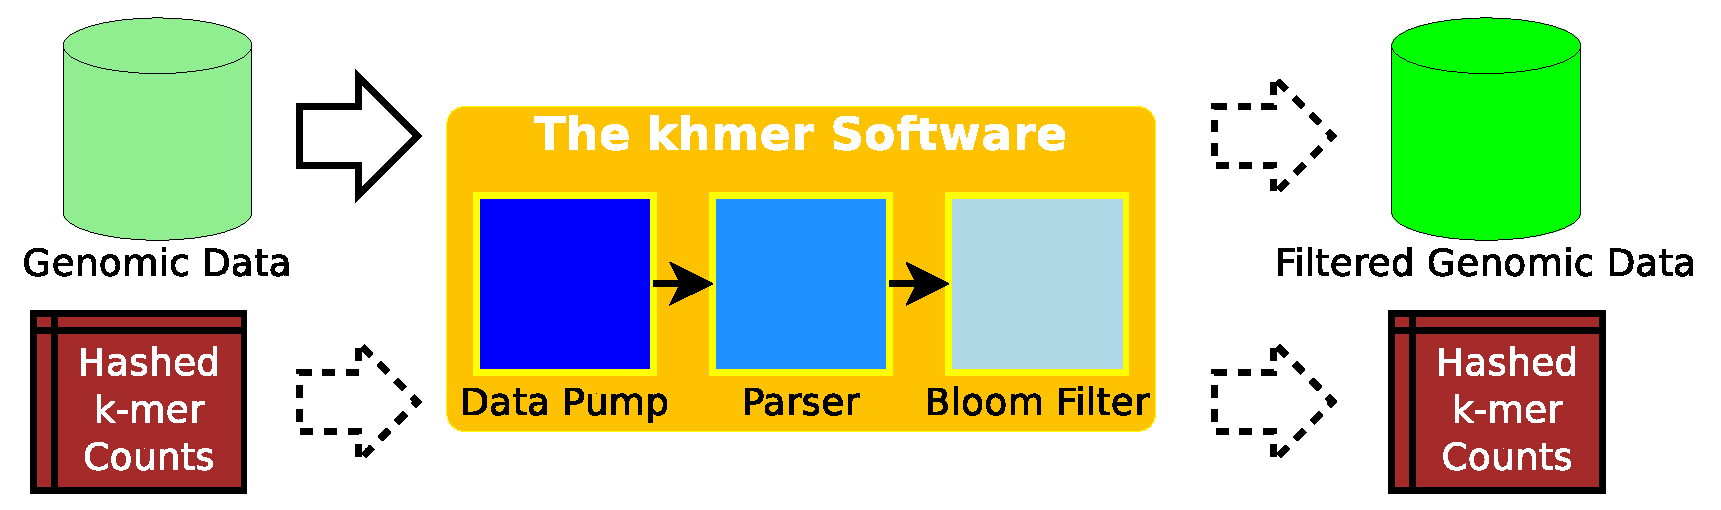
\includegraphics[scale=0.4]{data_flow.eps}
\caption{Data Flow through the khmer Software}
\label{khmerDataFlow}
\end{figure}

Lots and lots of data (potentially terabytes) must be moved from disk to memory by the software. Having an efficient data pump is crucial, as the input throughput from storage may be 3 or even 4 orders of magnitude less than the throughput for data transfer involving RAM. For some kinds of data files, a decompressor must be used. In either case, a parser must be able to work efficiently with the resultant data. The parsing task revolves around variable-length lines, but also must account for invalid genomic reads and what are known as paired reads. Each genomic read is broken up into a set of overlapping k-mers and each k-mer is registered with or compared against the Bloom filter. If a previously stored Bloom filter is being updated or used for comparison, then it must be loaded from storage. If a Bloom filter is being created for later use or updated, then it must be saved to storage.\comment{Refer explicitly to the figure.}

The data pump always performs sequential access on files and can potentially be asked to read large chunks of data at one time. With this in mind, the following are some of the questions which come to mind:
\begin{itemize}
\item Are we fully exploiting the fact that the data is accessed sequentially?
\item Are enough pages of data being prefetched into memory to minimize access latency?
\item Can asynchronous input be used instead of synchronous input?
\item Can we efficiently bypass system caches to reduce buffer-to-buffer copies in memory?
\item Does the data pump expose data to the parser in a manner that does create any unnecessary accessor or decision logic overhead?
\end{itemize}

%RCK - These bits here are the main issues at hand. Consider moving this list (and perhaps the one above) up to the beginning of the Architecture section, perhaps as an introductory teaser to give the reader an idea of what they should be paying attention to. Consider the following pattern: Express the problem; Describe the specifics involved; Explain how the problem was addressed, bullet by bullet.
Some considerations, regarding parser efficiency, are:
\begin{itemize}
\item Have we minimized the number of times that the parser is touching the data in memory?
\item Have we minimized the number of buffer-to-buffer copies while parsing genomic reads from the data stream?
\item Have we minimized the function call overhead inside the parsing loop?
\item Is DNA sequence validation being done as efficiently as possible?
\end{itemize}

For iterating over the k-mers in a genomic read and hashing them, we could ask:
\begin{itemize}
\item Can the k-mer iteration mechanism be optimized for both memory and speed?
\item Can the Bloom filter hash functions be optimized in any way?
\item Have we minimized the number of times that the hasher is touching the data in memory?
\item Can we increment hash counts in batches to exploit a warm cache?
\end{itemize}

%RCK - This whole section seems to be covering too much ground and too shallowly. You should narrow the focus onto a couple of the primary issues and then cover them in depth.

\section{Profiling and Measurement}

Simply reading the source code with an eye on performance revealed a number of areas for improvement. However, we wanted to systematically quantify the amount of time spent in various sections of the code. To do this, we used several profilers: the GNU Profiler (gprof) and the Tuning and Analysis Utilities (TAU). We also created instruments within the source code itself, allowing a fine granularity view of key performance metrics.

\subsection{Code Review}

Blindly applying tools to measure a system (software or otherwise) is rarely a good idea. Attempting to gain some understanding of the system before measuring it is usually a good idea. To this end, we reviewed the code by eye first.

Manually tracing the execution paths of an unfamiliar code is a good idea. (One of the authors, Eric McDonald, was new to the khmer software at the time he joined the project and he did this.) While it is true that profilers (and other tools) can generate call graphs, those graphs are only abstract summaries. Actually walking the code paths and seeing the function calls is a much more immersive and enlightening experience. Debuggers can be used for such walks, and are indeed useful in this regard, but they can be tedious to use, as often there are many lines that one wishes to skip and alternate execution paths one wants to explore. Using an editor with multiple display panes works quite well. Four display panes can often simultaneously capture all of the information a person needs to know - and is mentally capable of handling - at any given point.

The code review showed a number of things, some, but not all, of which were later revealed by profiling tools. Some of the things we noticed were:

\begin{itemize}
\item Highest traffic expected in k-mer counting logic.
\item Redundant calls to the \texttt{toupper} function in the highest traffic regions of the code.
\item Input of genomic reads performed line-by-line and on demand and without any readahead tuning.
\item A copy-by-value of the genomic read struct performed for every genomic read parsed and accepted as valid.
\end{itemize}

\subsection{Tools}

Profiling tools primarily concern themselves with the amount of time spent in any particular section of code. To measure this quantity, they inject instrumentation into the code at compile time. This instrumentation does change the size of functions, which may affect inlining during optimization. The instrumentation also directly introduces some overhead on the total execution time; in particular, the profiling of high traffic areas of code may result in a fairly significant overhead. So, if you are also measuring the total elapsed time of execution for your code, you need to be mindful of how profiling itself affects this. To gauge this, a simple external data collection mechanism, such as \texttt{/usr/bin/time}, can be used to compare non-profiling and profiling execution times for an identical set of optimization flags and operating parameters.

The size of the input data is not the only factor affecting the execution time of the khmer software. Choosing a smaller value of \texttt{k} will result in more k-mers per genomic read. This means that the k-mer counting logic will be exercised more. Any overhead associated with that logic, such as from profiling instrumentation, will thus scale inversely proportional to \texttt{k}. We, therefore, made measurements with execution at a couple of different k-mer lengths to understand the impact of this scaling. (One thing to keep in mind is that $k = 20$ or thereabouts was found to be ideal for use in the abundance-filtering approach that the khmer software pioneered. However, for most of our performance tests, we used $k = 30$ because of the quicker execution times.) For $k = 20$, we found that unprofiled code ran about 19\% faster than profiled code, and, for $k = 30$, that unprofiled code ran about 14\% faster than profiled code.

The GNU Profiler, gprof \citep{web:gprof}, is one of the tools which we used. This profiler relies upon a compiler to instrument the source code and a linker to link in some additional profiler-support logic, as appropriate. The \texttt{-pg} flag is used to enable profiling when using the GNU toolchain; other toolchains, such as those provided by Intel or PGI, also have switches for enabling gprof-compatible profiling. (Some compiler vendors in the Unix world also supply their own profiling tools and provide switches for supporting those, in addition to the gprof "standard".) When the compiled code is executed, it accumulates data about how much time is spent in particular functions. Upon completion of execution, this data is dumped to an output file, commonly called \texttt{gmon.out}, which can then be analyzed by the gprof tool proper.

Prior to any performance tuning, our profiling data showed that the k-mer counting logic was the highest traffic portion of the code, just as we predicted. What was a little surprising was how significant of a fraction it was, contrasted to I/O operations against storage. Given that our trial data sets were about 500 MB and 5 GB, we did not anticipate seeing much in the way of cache effects. Indeed, when we controlled for cache effects, we found that they did not amount to more than a couple of seconds at most and were thus not much larger than the error bars on our total execution times. This left us with the realization that I/O was not our only bottleneck.

Once we began parallelizing the khmer software, we wrote some driver programs, which used OpenMP \citep{web:OpenMP}, to test our parallelization of various components. While gprof is good at profiling single-threaded execution, it lacks the ability to trace per-thread execution when multiple threads are in use and it does not understand parallelization machinery, such as OpenMP. For C/C++ codes, OpenMP parallelization is determined by compiler pragmas. GNU C/C++ compilers, in the version 4.x series, honor these pragmas if supplied with the \texttt{-fopenmp} switch. When OpenMP pragmas are being honored, the compilers inject thread-handling instrumentation at the locations of the pragmas and around the basic blocks or other groupings with which they are associated.

As gprof could not readily give us the per-thread reporting and the OpenMP support that we desired, we turned to another tool. This was the Tuning and Analysis Utilities (TAU) \citep{web:TAU} from a collaboration led by the University of Oregon. There are a number of parallel profiling tools out there - many of them focus on programs using MPI (Message Passing Interface) libraries, which are popular for some kinds of scientific computing tasks. TAU supports MPI profiling as well, but as MPI is not really an option for the khmer software in its current manifestation, we ignored this aspect of TAU. Likewise, TAU is not the only tool available for per-thread profiling. The combination of per-thread profiling and the ability to integrate closely with OpenMP is one of the reasons that it was appealing to us. TAU is also entirely open source and not tied to any one vendor.

Whereas gprof relies solely upon instrumentation injected into source code at compile time (with some additional bits linked in), TAU not only provides this, but provides other instrumentation options as well. These options are library interposition (primarily used for MPI profiling) and dynamic instrumentation of binaries. To support these other options, TAU provides an execution wrapper, called \texttt{tau\_exec}. Compile-time instrumentation of source code is supported via a wrapper script, called \texttt{tau\_cxx.sh}.

TAU does not fully support all of its profiling facilities directly out of the box. To get tight OpenMP integration, for example, TAU needs to be configured and built with support for OPARI. Similarly, to use the performance counters exposed by newer Linux kernels, it needs to configured and built with support for PAPI. Also, once TAU is built, you will likely want to integrate it into your build system for convenience. For example, we setup our build system to allow the \texttt{tau\_cxx.sh} wrapper script to be used as the C++ compiler when TAU profiling is desired. If you attempt to build and use TAU, you will definitely want to read the documentation. While much more powerful than gprof, it is not nearly as facile or intuitive.

\subsection{Manual Instrumentation}

Examining the performance of a piece of software with independent, external profilers is all well and good, but sometimes it is more convenient to get the software to tell you certain numbers itself. Also, manual instrumentation can be less intrusive than automatic instrumentation, since you directly control what gets observed. To this end, we created an extensible framework to internally measure things such as throughputs, iteration counts, and timings around atomic or fine-grained operations within the software itself. As a means of keeping us honest, we internally collected some numbers that could be compared with measurements from the external profilers.

For different parts of the code, we needed to have different sets of metrics. However, all of the different sets of metrics have certain things in common. One thing is that they are mostly timing data and that you generally want to accumulate timings over the duration of execution. Another thing is that a consistent reporting mechanism is desirable. Given these considerations, we provided an abstract base class, \texttt{IPerformanceMetrics}, for all of our different sets of metrics. The \texttt{IPerformanceMetrics} class provides some convenience methods: \texttt{start\_timers}, \texttt{stop\_timers}, and \texttt{timespec\_diff\_in\_nsecs}. The methods for starting and stopping timers measure both elapsed real time and elapsed per-thread CPU time. The third method calculates the difference between two standard C library \texttt{timespec} objects in nanoseconds, which is of quite sufficient resolution for our purposes.

To ensure that the overhead of the manually-inserted internal instrumentation is not present in production code, we carefully wrapped it in conditional compilation directives so that a build can specify to exclude it.

\section{Tuning}

Making software work more efficiently is quite a gratifying experience, especially in the face of trillions of bytes passing through it. Our narrative will now wander through the various measures we took to improve efficiency. We divide these into two parts: optimization of the reading and parsing of input data and optimization of the manipulation and writing of the Bloom filter contents.

\subsection{General Tuning}

Before diving into some of the specifics of how we tuned the khmer software, we would like to briefly mention some options for general performance tuning. These options can be broadly categorized as aggressive optimizations and \textit{profile-guided optimizations} (PGO) \citep{web:PGO}. Aggressive optimizations are optimizations which may introduce bugs into the compiled code because of the assumptions which underly them; they may also be specific to a particular CPU family. Profile-guided optimizations rely on profiling information to make more educated guesses on how to optimize a program during compilation and linking. Although we will provide a little more detail on some of these optimizations, we must mention that we have, at this stage in our project, avoided them in favor of targeted algorithmic improvements - improvements that benefit everyone across many different CPU architectures. Also, from the standpoint of build system complexity, aggressive optimizations can create portability issues and profile-guided optimizations add to the total number of moving parts which may fail. Given that we do not distribute pre-compiled executables for various architectures and that our target audience is usually not too savvy about the intricacies of software development or build systems, it is likely that we will continue avoiding these optimizations until we feel that the benefits outweigh the drawbacks.

Optimization of locality arranges frequently-associated functions near one another in the text segment of an executable to increase the chance that they will be fetched into cache together on the same memory pages. This reduces cache misses and hence additional fetches. Although the collection of timing data is gprof's bread-and-butter, it also records a call graph. Using both the call graph and the timing data, it can deduce which functions are frequently associated with one another and provide hints for manual profile-guided optimization of locality. (These hints are provided by the \texttt{-R} and \texttt{-r} switches respectively.) However, manually performing PGO can be tedious and misses out on what a compiler and linker with PGO support can do automatically. The GNU C and C++ compilers support automatic PGO, which includes not only localization but also branch reordering and function inlining based on empirical data, among other things. (The initial compilation must be performed with the \texttt{-fprofile-generate} switch. After execution of the instrumented code, recompilation must be done with the \texttt{-fprofile-use} switch, feeding in the profiling data that the executable produced.)

\subsection{Data Pump and Parser Operations}

Our measurements showed that the time spent counting k-mers dominated the time performing input from storage. Given that interesting fact, it may seem like we should have devoted all of our efforts to improving the Bloom filter's performance. But, taking a look at the data pump and parser was worthwhile for several reasons. One reason was that we needed to alter the design of the existing data pump and parser to accommodate their use by multiple threads to achieve scalability. Another reason was that we were interested in reducing memory-to-memory copies, which could impact the efficiency of the Bloom filter at its interface with the parser. A third reason is that we wanted to position ourselves to provide an aggressive readahead or prefetch of data, in case we were able to improve the efficiency of the k-mer counting logic to the point that input time became competitive with counting time. Unrelated to performance tuning, there were also issues with maintainability and extensibility.

As it turns out, all of the above reasons converged on a new design. We will discuss the thread-safety aspects of this design in more detail later. For now, we will focus upon the reduction of memory-to-memory copies and the ability to perform fairly aggressive prefetching of data.

Typically, when a program retrieves data from a block storage device, a certain number of the blocks are cached by the operating system, in case the blocks are needed again. There is some time overhead associated with this caching activity; also, the amount of data to prefetch into the cache cannot be finely tuned. Furthermore, the cache cannot be accessed directly by a user process and so must be copied from the cache into the address space of the user process. This is a memory-to-memory copy. 

Some operating systems, such as Linux, allow for their readahead windows to be tuned some. One can make calls to \texttt{posix\_fadvise} and \texttt{readahead} for a particular file descriptor, for example. However, these allow rather limited control and do not bypass caching. We are interested in bypassing the cache maintained by the OS. This cache actually can be bypassed if a file is opened with the \texttt{O\_DIRECT} flag. Using direct input is not entirely straightforward, as the reads from storage must be multiples of the storage medium's block size and must be placed into memory, which is address-aligned on a multiple of that same block size. This requires a program to perform housekeeping which a file system would normally do. We implemented direct input, including the necessary housekeeping. There are, however, some cases where direct input will not work or is otherwise undesirable. For those cases, we still attempt to tune the readahead window. Our access of storage is sequential and we can tell the operating system to read further ahead than it normally would by using \texttt{posix\_fadvise} to provide a hint.

Minimizing buffer-to-buffer copies is a challenge shared between the data pump and the parser. In the ideal scenario, we would like to read once from storage into our own buffer and then scan our buffer once per genomic read to demarcate a sequence with an offset and length within the buffer. However, the logic for managing the buffer is complex enough and the logic for parsing (accounting for our particular nuances) is complex enough that maintaining an intermediary line buffer is quite useful for programmer comprehension. To reduce the impact of this intermediary buffer, we encourage the compiler to fairly aggressively inline this portion of the code. We may ultimately eliminate the intermediary buffer if performance of this particular region of the code becomes a big enough issue, but that may come at the expense of an understandable software design.

\subsection{Bloom Filter Operations}

Recalling that we are working with sequences composed of an alphabet of four letters: A, C, G, and T, you might ask whether these are uppercase or lowercase letters. Prior to performance tuning the code was insensitive to case right up to the points where it validated the DNA string and where it generated the hash codes. At these points, it would make redundant calls to the C library's \texttt{toupper} function to normalize the sequences to uppercase, using macros such as the following:

\begin{verbatim}

#define is_valid_dna(ch) \
    ((toupper(ch)) == 'A' || (toupper(ch)) == 'C' || \
     (toupper(ch)) == 'G' || (toupper(ch)) == 'T')

\end{verbatim}

and:

\begin{verbatim}

#define twobit_repr(ch) \
    ((toupper(ch)) == 'A' ? 0LL : \
     (toupper(ch)) == 'T' ? 1LL : \
     (toupper(ch)) == 'C' ? 2LL : 3LL)

\end{verbatim}

If you read the manual page for the \texttt{toupper} function or inspect the headers for the GNU C library, you might find that it is actually a locale-aware function and not simply a macro. So, this means that there is the overhead of calling a potentially non-trivial function involved - at least when the GNU C library is being used. But, we are working with an alphabet of four ASCII characters. A locale-aware function is overkill for our purposes. So, not only do we want to eliminate the redundancy but we want to use something more efficient.

We decided to normalize the sequences to uppercase letters prior to validating them. (And, of course, validation happens before attempting to convert them into hash codes.) While it might be ideal to perform this normalization in the parser, it turns out that sequences can be introduced to the Bloom filter via other routes. So, for the time being, we chose to normalize the sequences immediately prior to validating them. This allows us to drop all calls to \texttt{toupper} in both the sequence validator and in the hash encoders.

Considering that terabytes of genomic data may be passing through the sequence normalizer, it is in our interests to optimize it as much as we can. One approach is:

\begin{verbatim}
#define quick_toupper( c ) (0x60 < (c) ? (c) - 0x20 : (c))
\end{verbatim}

For each and every byte, the above should execute one compare, one branch, and possibly one addition. Can we do better than this? As it turns out, yes. Note that every lowercase letter has an ASCII code which is 32 (hexadecimal 20) greater than its uppercase counterpart and that 32 is a power of 2. This means that the ASCII uppercase and lowercase characters differ by a single bit only. This observation screams "bitmask!"

\begin{verbatim}
c &= 0xdf; // quicker toupper
\end{verbatim}

The above has one bitwise operation, no compares, and no branches. Uppercase letters pass through unmolested; lowercase letters become uppercase. Perfect, just we wanted. For our trouble, we gained about a 13\% speedup.

Our Bloom filter's hash tables are... ``expansive''. To increment the counts for the hash code of a particular k-mer almost means hitting \texttt{N} different memory pages, where \texttt{N} is the number of hash tables allocated to the filter. In many cases, the memory pages which need to be updated for the next k-mer are entirely different than those for the current one. This can lead the much cycling of memory pages from main memory without being able to utilize the benefits of caching. If we have a genomic read with a 79-character long sequence and are scanning k-mers of length 20, and if we have 4 hash tables, then up to 236 (59 * 4) different memory pages are potentially being touched. If we are processing 50 million reads, then it is easy to see how costly this is. What to do about it?

One solution is to batch the hash table updates. By accumulating a number of hash codes for various k-mers and then periodically using them to increment counts on a table-by-table basis, we can greatly improve cache utilization. Initial work on this front looks quite promising and, hopefully, by the time you are reading this, we will have fully integrated this modification into our code. Although we did not mention it earlier in our discussion of measurement and profiling, \texttt{cachegrind}, a program which is part of the open-source Valgrind \citep{web:Valgrind} distribution, is a very useful tool for gauging the effectiveness of this kind of work.

\section{Parallelization}

With the proliferation of multi-core architectures in today's world, it is tempting to try taking advantage of them. However, unlike many other problem domains, such as computational fluid dynamics or molecular dynamics, our Big Data problem is essentially I/O-bound. Beyond a certain point, throwing additional threads at it does not help as the bandwidth to the storage media is saturated and the threads simply end up with increased blocking or I/O wait times. That said, utilizing some threads can be useful, particularly if the data to be processed is held in physical RAM, which generally has a much higher bandwidth than online storage. As discussed previously, we have implemented a prefetch buffer in conjunction with direct input. Multiple threads can use this buffer; more will be said about this below. I/O bandwidth is not the only finite resource which multiple threads must share. The hash tables used for k-mer counting are another one. Shared access to these will also be discussed below.

\subsection{Thread-safety and Threading}

Before proceeding into details, it may be useful to clear up a couple items about terminology. People often confuse the notion of something being thread-safe with that of something being threaded. If something is thread-safe, then it can be simultaneously accessed by multiple threads without fear of corrupted fetches or stores. If something is multi-threaded, then it is simultaneously operated by multiple threads of execution.

As part of our parallelization work, we remodeled portions of the C++ core implementation to be thread-safe without making any assumptions about a particular threading scheme or library. Therefore, the Python \texttt{threading} module can be used in the scripts which use the Python wrapper around the core implementation, or a C++ driver around the core could use a higher-level abstraction, like OpenMP as we mentioned earlier, or explicitly implement threading with \texttt{pthreads}, for example. Achieving this kind of independence from threading scheme and guaranteeing thread-safety, while not breaking existing interfaces to the C++ library, was an interesting software engineering challenge. We solved this by having portions of the API, which were exposed as thread-safe, maintain their own per-thread state objects. These state objects are looked up in a C++ Standard Template Library (STL) \texttt{map}, where thread identification numbers are the keys. The identification number for a particular thread is found by having that thread itself query the OS kernel via a system call. This solution does introduce a small amount of overhead from having a thread inquire about its identification number on every entry to a function exposed via the API, but it neatly avoids the problem of breaking existing interfaces, which were written with a single thread of execution in mind.

\subsection{Data Pump and Parser Operations}

The multi-core machines one encounters in the HPC world may have multiple memory controllers, where one controller is closer (in terms of signal travel distance) to one CPU than another CPU. These are \textit{Non-Uniform Memory Access} (NUMA) architectures. A ramification of working with machines of this architecture is that memory fetch times may vary significantly depending on physical address. As bioinformatics software often requires a large memory footprint to run, it is often found running on these machines. Therefore, if one is using multiple threads, which may be pinned to various \textit{NUMA nodes}, the locality of the physical RAM must be taken into consideration. To this end, we divide our prefetch buffer into a number of segments equal to the number of threads of execution. Each thread of execution is responsible for allocating its particular segment of the buffer. The buffer segment is administered via a state object, maintained on a per-thread basis.

\subsection{Bloom Filter Operations}

The Bloom filter hash tables cannot be split into separate copies among threads. Rather, a single set of tables must be shared by all of the threads. This implies that there will be contention among the threads for these resources. Memory barriers \citep{web:membar} or some form of locking are needed to prevent two or more threads from attempting to access the same memory location at the same time. We use atomic addition operations to increment the counters in the hash tables. These atomic operations \citep{web:atomics} are supported on a number of platforms by several compiler suites, the GNU compilers among those, and are not beholden to any particular threading scheme or library. They establish memory barriers around the operands which they are to update, thus adding thread-safety to a particular operation.

A performance bottleneck, which we did not address, is the time to write the hash tables out to storage after k-mer counting is complete. We did not feel that this was such a high priority because the write-out time is constant for a given Bloom filter size and is not dependent upon the amount of input data. For a particular 5 GB data set, which we used for benchmarking, we saw that k-mer counting took over six times as long as hash table write-out. For even larger data sets, the ratio becomes more pronounced. That said, we are ultiamtely interested in improving performance here too. One possibility is to amortize the cost of the write-out over the duration of the k-mer counting phase of operation. The URL-shortener site, bit.ly, has a counting Bloom filter implementation, called \texttt{dablooms} \citep{web:dablooms}, which achieves this by memory-mapping its output file to the hash table memory. Adopting their idea, in conjunction with batch updates of the hash tables, would effectively give us asynchronous output in bursts over a process' lifetime and chop off the entire write-out time from the end of execution. Our output is not simply tables of counts, however, but also includes a header with some metadata; implementing memory-mapping in light of this fact is an endeavor that needs to be approached thoughtfully and carefully.

\subsection{Scaling}

Was making the khmer software scalable worth our effort? Yes. Of course, we did not achieve perfectly linear speedup. But, for every doubling of the number of cores, we presently get about a factor of 1.9 speedup. We think that we can do even better by improving our access patterns around shared resources, such as the hash table memory, and by better streamlining the use of per-thread state objects. At some point, though, if we improve per-thread efficiency enough and improve the scaling factor enough, Amdahl's Law \citep{web:Amdahl} will rear its head. This is to say that I/O, plus some initialization and bookkeeping overhead, constitutes a serial portion of the software's execution. I/O can be made to scale somewhat via asynchronous reads and writes, but its bandwidth is ultimately finite and saturation will eventually be reached.

% TODO? Plot speedup curve.

\section{Conclusion}

The khmer software is a moving target. New features are being added to it, and we are working on incorporating it into various software stacks in use by the bioinformatics community. Like many pieces of software in academia, it started life as an exploratory programming exercise and evolved into research code. Correctness was and is a primary goal of the project. While performance and scalability cannot truly be regarded as afterthoughts, they yield precedence to correctness and utility. That said, our efforts regarding scalability and performance have produced good results, including speedups in single-threaded execution and the ability to significantly reduce total execution time by employing multiple threads. Thinking about performance and scalability issues led to the redesign of the data pump and parser components. Going forward, these components should be able to benefit not only from scalability but improved maintainability and extensibility.

We look forward to continuing the development of this software and hope to have an impact on the Big Data problem facing molecular biologists and bioinformaticians. We hope that you enjoyed reading about some high performance, open source software being employed in the sciences.

\bibliographystyle{plain}
\bibliography{references}
\end{document}

% vim: set ft=tex sw=4 sts=4:
